%
% 卒論レジュメフォーマット Ver.2.0 pLaTeX版
%
\documentclass[twocolumn]{jarticle} % 2段組のスタイルを用いている

\usepackage{wuse_resume}
\usepackage{url}	% \url{}コマンド用.URLを表示する際に便利
\usepackage[dvipdfmx]{graphicx}  % ←graphicx.styを用いてEPSを取り込む場合有効にする
			% 他のパッケージ・スタイルを使う場合には適宜追加
			
\usepackage[hang,small,bf]{caption}
\usepackage[subrefformat=parens]{subcaption}
\usepackage{here}

%%%%%%%%%%%%%%%%%%%%%%%%%%%%%%%%%%%%%%%%%%%%%%%%%%%%%%%%%%%%%%%%%%%%%%%%

%%
%% タイトル,学生番号,氏名などを設定する
%%

\タイトル{オブジェクトの動作に基づくScratch作品の直観的検索手法}
\研究室{ソーシャルソフトウェア工学}
\学生番号{60236238}
\氏名{福地 ユキ}

\概要{%
ビジュアルプログラミング言語Scratchにおいて,ユーザはオンラインサービス上に公開された他者の作品を
キーワードで検索し,参照することで実装方法を学習する.
しかし,ユーザの持つ動作のイメージをキーワードに変換することは難しく,
作品のタイトルや説明文に動作のキーワードを含まない作品は検索結果に表示されないため,
作品検索は容易ではない.
本論文ではScratch作品の検索を容易にするために,
キーワードによる検索ではなく動作のイメージを入力とする直感的な検索手法を提案する.
}

\キーワード{Scratch}
\キーワード{コード検索}
\キーワード{時系列解析}
\キーワード{物体追跡}
\キーワード{画像検索}

%%%%%%%%%%%%%%%%%%%%%%%%%%%%%%%%%%%%%%%%%%%%%%%%%%%%%%%%%%%%%%%%%%%%%%%%

%% 以下の3行は変更しない

\begin{document}
\maketitle
\thispagestyle{empty} % タイトルを出力したページにもページ番号を付けない

%%%%%%%%%%%%%%%%%%%%%%%%%%%%%%%%%%%%%%%%%%%%%%%%%%%%%%%%%%%%%%%%%%%%%%%%

%%
%% 本文 - ここから
%%

\section{はじめに}
ビジュアルプログラミング言語のScratchでは,
ユーザが制作したプログラム作品をオンラインサービス上に公開可能である.
オンラインサービス上には,膨大な数の作品が公開されており,
ユーザは他者の作品を参照することで多様な実装方法を学習する\cite{spfa}.
参照する他者の作品を探し出すために,ユーザはキーワード検索を行う.
しかし,ユーザがイメージする動作を言語化することは難しく,
動作に関するキーワードをタイトルや説明文に含まない作品は検索不可能であるため,
イメージに類似する動作を含む作品の検索は容易ではない\cite{wild}.
動作のイメージを入力とする検索を実現することで,作品検索を容易にできると考える.
本論文では,マウスを用いて動作のイメージを入力する
Scratch作品の直観的検索手法を提案する.

\section{オブジェクトの動作に基づくScratch作品検索手法}
\subsection{手順1: オブジェクトの座標変化を取得}
手順1では,入力の動作イメージと検索対象作品に含まれる動作の座標変化データを取得する.
\subsubsection{動作イメージの入力}
ユーザの持つ動作のイメージをマウスで描画することによって入力する.
動作のイメージを描画中,0.2秒ごとにマウスの座標を取得する.
取得した座標を入力の座標変化データとする.

\subsubsection{検索対象作品に含まれるオブジェクトの動作}
\paragraph{検索対象作品の収集}
Webアプリケーションの自動テストツールSelenium\footnote{https://www.selenium.dev/}
を用いて,検索対象作品の実行結果のスナップショットを0.2秒ごとに収集する.

\paragraph{画像認識による座標変化データ取得}
収集した各作品のスナップショットに含まれるオブジェクトの座標位置を,
SIFT(Scale-Invariant Feature Transform)を用いた画像認識によって取得する.
Scratch では,オブジェクトの色や回転・拡大縮小を自由に変更できることから,
照明変化や回転・拡大縮小に頑健であるSIFTを採用する.

\subsection{手順2: 座標変化同士の距離を算出}
\subsubsection{座標変化データの正規化}
入力と検索対象動作の座標が離れていても,
動作の軌跡が類似していれば類似動作として抽出を行うため,
手順1で取得した時系列データを最小値0,最大値1に正規化する.

\subsubsection{DTW距離の算出}
入力と各動作の座標変化の類似性を測るために,
2つの時系列データの距離を算出する動的時間伸縮法(DTW: Dynamic time warping)によって距離を算出する.
異なる長さの時系列データ同士でも距離算出が可能であるため,DTWを採用する.

\section{類似動作を抽出可能な距離の分析}\label{chap:fig-tab-exp}
類似動作を抽出可能な距離を明らかにするために,
複数の入力を行い,
DTW距離の算出結果について定量分析と定性分析を行う.
また,提案手法による作品検索の精度を明らかにするために,
ランキング指標を用いた検索評価を行う.

\subsection{検索データセット}
Aivaloglouらの公開データセット\footnote{https://github.com/TUDelftScratchLab/ScratchDataset}のうち,
13,437件のScratch作品を検索対象とする.

\subsection{入力}
直線移動や曲線移動をする4つの動作を入力する.

\begin{figure}[H]
    \centering
    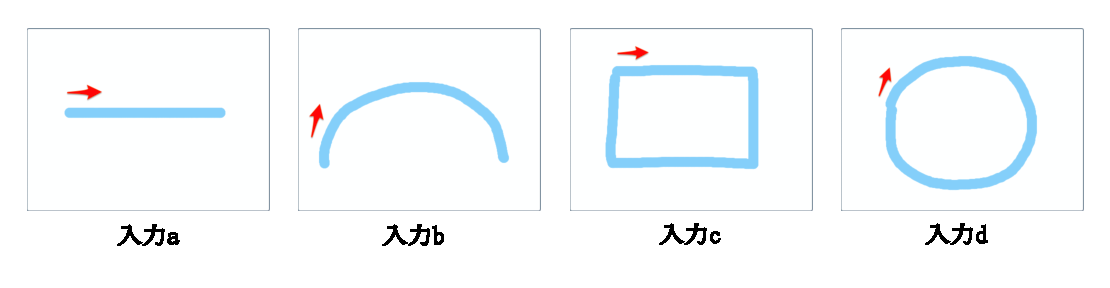
\includegraphics[width=8cm]{resume-input.eps}
    \caption{分析で用いる4つの入力}
    \label{systemdisplay}
\end{figure}

\subsection{定量分析}
\label{teiryou}
類似しない動作が抽出される距離を明らかにするために,各入力に対する距離算出結果を昇順に並べ,
ある2点の傾きが収束する値を求める.
傾きが0.5未満となり,動作を目視で確認した結果移動方向が入力と異なっている場合,
その時点の距離を収束する値とする.
各入力に対して定量分析を行なった結果を表\ref{quantitativeresult}に示す.
結果の距離以下の動作を,続く\ref{teisei}節で実施するアンケートで提示する.
        
\begin{table}
    \caption{移動方向が異なる動作が抽出される距離}
    \label{quantitativeresult}
    \centering
    \begin{tabular}{c|c|c|c}
    \hline
    入力 & 距離 \\
    \hline \hline
    a & 4.4 \\
    \hline
    b & 3.2 \\
    \hline
    c & 6.9 \\
    \hline
    d & 7.9 \\
    \hline
    \end{tabular}
\end{table}

\subsection{定性分析}
\label{teisei}
類似動作を抽出可能な距離を明らかにするために,
入力と各検索対象動作の DTW 距離算出結果から距離の異なる複数の動作を提示し,
動作の類似性をアンケートで評価する.
動作の類似性は,4段階のリッカート尺度(1: 類似する,2: やや類似する,3: やや類似しない,4: 類似しない)
で評価し,初めて回答者全員が「4: 類似しない」を選択した距離未満を,類似動作を抽出可能な距離とする.
「1: 類似する」以外を選択した場合,理由を記述する.
各入力における類似動作を抽出可能な距離の結果を,表\ref{result}に示す.
類似動作を抽出可能な距離は入力によって異なることが明らかとなった.
入力a,c,dの結果は,それぞれ4.3未満,4.1未満,4.5未満となったのに対し,
入力bのみ2.2未満と距離が近くなっている.

\subsection{検索評価}
\label{ranking}
本論文で提案する検索手法の精度を評価するために,各入力に対する距離算出結果のうち,
距離の近い上位20件を用いて\ref{teisei}節と同様にアンケートを実施した.
検索評価のために,MRR(Mean Reciprocal Rank)を算出する.
アンケートの結果から,初めて回答者全員が質問1に対して「1: 類似する」を選択した動作を正解とし,
MRRを算出した結果0.88となった.

\section{考察}
\subsection{動作に基づく検索手法の実用性}
\ref{teisei}で実施した定性分析の結果から,
見た目と実際の座標変化に差異がある動作が存在し,その原因が画像認識にずれがあることや,
移動方向は類似するが曲線(直線)移動ではなく直線(曲線)移動をする動作が抽出され,
その原因が座標変化取得の時間間隔にあることから,検索の精度向上のために改善が必要であることが明らかとなった.
しかし,いずれの入力においても回答者全員が類似すると判断する動作が複数存在しており,
\ref{ranking}節の検索評価の結果からランキング上位に類似動作が出現することが期待できるため,
動作に基づく作品検索手法は実用性があると考える.

\subsection{抽出した類似動作のプログラム}
動作に基づく作品検索を行うことで,類似動作の多様な実装方法を検索可能であることが明らかになった.
実装方法の異なる類似動作を提示することは,プログラムの実装方法やより品質の良い実装の両方の学習に繋がり,
特に初学者も多く利用しているScratchにおいて有用であると考える.

\section{おわりに}
本論文で提案した手法により,
動作のイメージを入力とした類似動作の検出が可能であることが明らかとなった.
また,動作に基づく検索により,類似動作の多様な実装方法を検索可能であることが明らかになったため,
他者の作品を参照することによる実装方法学習の支援を期待する.

\begin{table}
    \caption{類似動作を抽出可能な距離}
    \label{result}
    \centering
    \begin{tabular}{c|c}
    \hline
    入力 & 距離(未満) \\
    \hline \hline
    a & 4.3 \\
    \hline
    b & 2.2 \\
    \hline
    c & 4.1 \\
    \hline
    d & 4.5 \\
    \hline
    \end{tabular}
\end{table}


%%
%% 本文 - ここまで
%%

%%%%%%%%%%%%%%%%%%%%%%%%%%%%%%%%%%%%%%%%%%%%%%%%%%%%%%%%%%%%%%%%%%%%%%%%

%%
%% 参考文献
%%

\begin{thebibliography}{9}	% {9}は文献に付ける通し番号の表示に必
				% 要な幅を指定している.10件以上になる
				% 場合には2桁の数({99}など)を指定する.
				
\bibitem{spfa}
Mitchel Resnick, John Maloney, Andr\'{e}s Monroy-Hern\'{a}ndez, Natalie Rusk, Evelyn Eastmond, Karen Brennan, 
Amon Millner, Eric Rosenbaum, Jay Saul Silver, Brian S Silverman, Yasmin Bettina Kafai,
Scratch: Programming for all,
Communications of the ACM, Vol.52, No.11, pp.60-67, 2009.

\bibitem{wild}
Aniket Dahotre, Yan Zhang, Christopher Scaffidi,
A qualitative study of animation programming in the wild,
ESEM'10: Proceedings of the 2010 ACM-IEEE International Symposium on Empirical Software Engineering and Measurement,
No.29, pp.1-10, 2010.

\end{thebibliography}

%%%%%%%%%%%%%%%%%%%%%%%%%%%%%%%%%%%%%%%%%%%%%%%%%%%%%%%%%%%%%%%%%%%%%%%%

\end{document}
